% ═══════════════════════════════════════════════════════════════════════════════
% ZOMBI2 — How the gene-family coupling model works (implementation explainer)
% ═══════════════════════════════════════════════════════════════════════════════
\documentclass[11pt]{article}
\usepackage[T1]{fontenc}
\usepackage[margin=0.9in]{geometry}
\usepackage{amsmath, amssymb}
\usepackage{xcolor}
\usepackage{tikz}
\usetikzlibrary{arrows.meta, positioning, calc}
\usepackage{enumitem}
\usepackage{tcolorbox}
\tcbuselibrary{breakable, skins}
\usepackage{listings}
\usepackage{fancyhdr}
\usepackage[hidelinks]{hyperref}
\usepackage{titlesec}
\titlespacing*{\section}{0pt}{6pt}{2pt}
\setlist{nosep, leftmargin=1.3em}

\definecolor{mainblue}{RGB}{41, 54, 122}
\definecolor{maingreen}{RGB}{98, 175, 74}
\definecolor{mainred}{RGB}{183, 53, 45}
\definecolor{boxbg}{RGB}{245, 247, 252}
\definecolor{codebg}{RGB}{247, 247, 249}

\newtcolorbox{conceptbox}[1][]{colback=boxbg, colframe=mainblue, fonttitle=\bfseries,
  title=#1, breakable, sharp corners=south, boxrule=0.8pt, left=6pt, right=6pt, top=4pt, bottom=4pt,
  before upper={\parindent=0pt}}
\newtcolorbox{intuitionbox}[1][]{colback=maingreen!6, colframe=maingreen!60!black, fonttitle=\bfseries,
  title=#1, breakable, sharp corners=south, boxrule=0.8pt, left=6pt, right=6pt, top=4pt, bottom=4pt,
  before upper={\parindent=0pt}}
\newtcolorbox{warningbox}[1][]{colback=mainred!5, colframe=mainred!60!black, fonttitle=\bfseries,
  title=#1, breakable, sharp corners=south, boxrule=0.8pt, left=6pt, right=6pt, top=4pt, bottom=4pt,
  before upper={\parindent=0pt}}

\lstdefinestyle{py}{basicstyle=\ttfamily\scriptsize, backgroundcolor=\color{codebg},
  keywordstyle=\color{mainblue}\bfseries, commentstyle=\color{maingreen!60!black},
  stringstyle=\color{mainred}, language=Python, showstringspaces=false, frame=none,
  xleftmargin=6pt, aboveskip=3pt, belowskip=2pt}

\pagestyle{fancy}\fancyhf{}
\fancyhead[L]{\small\textcolor{mainblue}{ZOMBI2 --- Gene-family coupling model}}
\fancyhead[R]{\small\textcolor{mainblue}{\texttt{zombi2.coupling}}}
\renewcommand{\headrulewidth}{0.4pt}
\setlength{\parskip}{2pt}
\setlength{\emergencystretch}{2.5em}

\title{\vspace{-1.5cm}{\Large\textcolor{mainblue}{\textsc{How the gene-family coupling model works}}}\\[0.2em]
  {\normalsize A Potts/Ising model of non-independent gene families in ZOMBI2}}
\author{}\date{\vspace{-1.2cm}}

\begin{document}
\maketitle\thispagestyle{fancy}\vspace{-0.7cm}

\noindent
By default ZOMBI2 evolves every gene family independently, so the phylogenetic profile it
emits---the \emph{families $\times$ species} presence/copy-number matrix---has rows that
correlate \emph{only} through the shared species tree. Real genomes correlate through
\emph{function}: families in one pathway or complex tend to be present or absent
\emph{together}, the signal that phylogenetic-profiling and inverse-Potts methods exploit.
The \texttt{zombi2.coupling} model is the forward, \emph{generative} counterpart: you
prescribe pairwise couplings, and it produces profiles that carry that co-occurrence
structure as a known ground truth for benchmarking those inference methods.

% ─────────────────────────────────────────────────────────────────────────────
\section*{\textcolor{mainblue}{1\quad The model}}
Fix a panel of $N$ gene families. Inside one genome, their presence/absence is an Ising
vector $\sigma\in\{0,1\}^N$ ($\sigma_i=1$ means family $i$ is present). Two ingredients set
how a family behaves: a \emph{field} $h_i$ (its intrinsic tendency to be retained) and, for
each pair, a \emph{coupling} $J_{ij}$ (how much $i$ and $j$ ``like'' to co-occur). Together
they give the \emph{local field} that family $i$ feels from everyone else:

\begin{conceptbox}[The two rate rules]
\vspace{-2pt}
\[
  f_i(\sigma)=h_i+\sum_{j}J_{ij}\,\sigma_j
  \qquad\Longrightarrow\qquad
  \underbrace{\text{loss}_i=\ell_0\,e^{-\beta f_i}}_{\text{coupled}},
  \qquad
  \underbrace{\text{gain}_i=\text{horizontal transfer}}_{\text{field-blind}}
\]
\vspace{-6pt}
\begin{itemize}
\item \textbf{Loss carries the coupling.} A \emph{present} family is lost at rate
  $\ell_0\,e^{-\beta f_i}$. A present partner with $J_{ij}>0$ raises $f_i$ and so
  \emph{lowers} $i$'s loss (they protect one another); $J_{ij}<0$ raises loss (they exclude
  one another); $J_{ij}=0$ is independence. $h_i$ is the solo bias ($h_i\!\gg\!0$ is a
  near-universal ``hub'' gene); $\beta$ is a global coupling strength.
\item \textbf{Gain is horizontal transfer.} A lost family returns only when a donor that
  still has it transfers a copy in---the ordinary, function-blind HGT event.
\end{itemize}
\end{conceptbox}

The coupling never appears in the gain step. Instead it acts through \emph{differential
retention}: transfer sprays families around blindly, and the coupled loss then \emph{keeps}
a newly acquired family where its partners are present (high $f_i$, slow loss) and
\emph{purges} it where they are absent (low $f_i$, fast loss). That selective retention of
horizontally-acquired genes is what writes $J$ into the final profiles.

% ─────────────────────────────────────────────────────────────────────────────
\section*{\textcolor{mainblue}{2\quad Why co-occurrence emerges}}
\begin{minipage}[t]{0.60\textwidth}
\vspace{2pt}
Take two families with a strong positive coupling. While both are present, each raises the
other's field, so both are lost slowly---they persist \emph{together}. The moment one is
lost, the other loses its protection, its loss rate jumps, and it tends to follow: losses
\emph{cascade}, giving all-or-nothing pathways. Across many lineages some keep the pair and
some lose it, so the two rows of the profile line up---positive correlation. Flip the sign
of $J$ and the same logic runs backwards: each family's presence \emph{raises} the other's
loss, so they end up in different genomes (avoidance, negative correlation). With $J=0$ the
rows are independent given the tree.
\end{minipage}\hfill
\begin{minipage}[t]{0.36\textwidth}
\vspace{0pt}
\centering
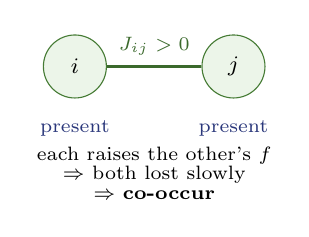
\begin{tikzpicture}[font=\footnotesize, node distance=6mm]
  \node[circle, draw=maingreen!70!black, fill=maingreen!12, minimum size=8mm] (A) {$i$};
  \node[circle, draw=maingreen!70!black, fill=maingreen!12, minimum size=8mm, right=12mm of A] (B) {$j$};
  \draw[maingreen!60!black, very thick] (A)--(B) node[midway, above, font=\scriptsize]{$J_{ij}>0$};
  \node[below=1.5mm of A, font=\scriptsize, text=mainblue] {present};
  \node[below=1.5mm of B, font=\scriptsize, text=mainblue] {present};
  \node[below=9mm of $(A)!0.5!(B)$, align=center, font=\scriptsize]
    {each raises the other's $f$\\[-1pt]$\Rightarrow$ both lost slowly\\[-1pt]$\Rightarrow$ \textbf{co-occur}};
\end{tikzpicture}
\end{minipage}

% ─────────────────────────────────────────────────────────────────────────────
\section*{\textcolor{mainblue}{3\quad How it plugs into ZOMBI2}}
ZOMBI2's forward simulator already hands each rate model the \emph{whole} genome (through its
\texttt{event\_weights} method). The coupling is therefore a single new rate
model, \texttt{PottsRates}, and \textbf{nothing else changes}---not the simulator, the
genome, the event types, nor the output:

\begin{enumerate}
\item read the presence vector $\sigma$ straight off the genome;
\item for every \emph{present} family emit a loss weight $\ell_0 e^{-\beta f_i}$; add one
  field-blind transfer channel for the gain side;
\item the simulator recomputes the branch's weights after \emph{every} event, so the field
  $f_i$ is always current---i.e.\ genuine state-dependent (Glauber-style) dynamics along the
  tree, for free.
\end{enumerate}
Because a custom rate model breaks per-family independence it runs on the pure-Python engine
(the Rust fast path could not apply anyway); the cost is $O(N+\text{nnz}(J))$ per event.

\begin{warningbox}[One caveat worth stating plainly]
Because the gain channel is \emph{field-blind}, the process has \textbf{no exact Boltzmann
stationary distribution}---this is an \emph{approximate} Potts generator by design (a lost
gene returns only from a donor that has it, which is the honest biology). Consequently,
couplings recovered from the profiles track the injected $J$ in \textbf{sign and rank, not as
an exact multiple}. Separately, on an ordinary birth--death tree even \emph{uncoupled}
families co-occur through shared ancestry (clade-restricted loss), so raw correlation is
confounded by phylogeny---exactly why real inference corrects for the tree, and why the
validation below uses a near-star tree to isolate the coupling.
\end{warningbox}

% ─────────────────────────────────────────────────────────────────────────────
\section*{\textcolor{mainblue}{4\quad Using it, and how we check it}}
\begin{lstlisting}[style=py]
from zombi2 import simulate_species_tree, BirthDeath, pathway_blocks, simulate_coupled

tree = simulate_species_tree(BirthDeath(1.0, 0.2), n_tips=100, age=6.0, seed=1)
spec = pathway_blocks([3, 3], within=3.0, between=-1.0,   # two co-occurring pathways,
                      h=2.0, base_loss=1.0, transfer=0.2)  # mutually exclusive
res  = simulate_coupled(tree, spec, seed=1)
res.profiles     # N x species matrix, ground-truth couplings baked in
\end{lstlisting}

\noindent
Couplings can also be supplied as a dense matrix or a sparse edge list
(\texttt{CouplingSpec.from\_dense} / \texttt{.from\_edges}). The test suite validates two
things:
(i)~the loss rate equals $\ell_0 e^{-\beta f_i}$ exactly---a positive partner lowers a
family's loss, a negative partner raises it; and (ii)~\emph{inject~$\to$~recover}---simulate
under a known $J$ and confirm the profiles show the prescribed structure ($+J\Rightarrow$
co-occurrence, $-J\Rightarrow$ avoidance, $J=0\Rightarrow$ none), measured on a near-star
tree so the signal is the coupling, not the phylogeny.

\end{document}
